\documentclass[../main/main.tex]{subfiles}

\newdate{date}{05}{11}{2020}


\begin{document}

\marginpar{ \textbf{Lecture 11.} \\  \displaydate{date}. \\ Compiled:  \today.}


TOday we will take into account something which is quite common. Usually diseases does not spread in isolation, but interact with other diseases.

Most of the ifnection diseases that we have seen write now, there are different variants circulating for the same disease. For instance, for the season influenza we have different virus which are similar, we have a family of virus. These virus interact between each other.

It is extremely important that a disease can be with a several variants.


Let us consider in which we have two different diseases which cooperate. One disease boost the spread of the other one. The map represent the spread of tubercolosis in 1990. Tubercolosi is a disease with a very strong latent period, the disease can be in a latent state for many many years. We have the same map in 2005. We note that the disease exploit especially in the south.
The number almost doubles. The reason is that HIV reach africa. HIV is a disease which compromise your immune system, so your immune system is less efficient: the probability of getting any other disease is higher than the normal.

When they got HIV the immune system go down and tubercolosi activate. The numbers represent the fraction of pations which get HIV and tubercolosis. SO HIV is helping a lot for the spread of tubercolosi.
This was the first example of interaction of two diseases.


The other case we can have is \textbf{competition} as seasonal influenza. We have the distribution of the different influenza virus which circulates for the season. We have a cake plot in which we see that a certain number of people got this type of influenza (light blue). We can see that the influenza curve is a mixture of several different types.

Each year seasonal influenza is caused by different virus.

Our immune system has a sort of memory. So if we got one disease we can get the same the next year.

So actually the suscpetible population is just a reduced fraction. This is why every year we do not have a huge pandemic of influenza.

There is another case \textbf{evolution} when we have virus which mutate a lot.
For instance HIV is an extremely volatile virus so it can mutate a lot. We have different types and subtypes. We can see how these subtypes are distributed on different areas.

We are gonna focus only on the simple setting in which we consider competition and cooperation between diseases. How is it possible to model these kind of interactions?
The simplest solution is to couple different dynamics.

For instance, in the simplest state we can couple SIS and SIR dynamics.
We have twice the number of states (we take into account all the possible combinations). Each disease its gonna have its own parameter.
We need at least some parameter which encode this kind of interaction between diseases.

Let us see one of this model. Let us consider a classical heterogeneous mean-field in which we have two different diseases.
We have also two different networks in which diseases spread.
For instance, one disease diffuse in an oral way, while the other one by blood. So the network can be different from one disease to the other. So, each network has its own degree distribution and we have to use the joint distribution.

Since we are doing a degree based mean field, in this case we have four different equations for all couple of different disease. So, the state of the system is represented by these four variables.

Hence, we have to take into account (to represent a general model) this interaction effect. We introduce the \textbf{modified susceptibility}. For instance, having one disease make the individual more susceptible than the others.

If we want that this framework as general as possible, we have to consider that the suscpebility can be modiefied and also the probability of getting the diseas. If I am being infected of one disease makes me more/less infected (depending if the parameter is positive or not).

The third interaction that you can have is on the recovery. If I have another disease probably my recovery time will be large. If \( \eta  \) is smaller than 1, my recovery period will be larger (cooperative effects of the diseases), instead if it is larger than 1 we have the competitive.

These are all the possible interactions we can have in this simple model. These are all the possibilities that we can have. The normal ifnectiion and the recovery process. Then, we have an increase in suscpetibility, in infectivity. You can play with these parameter as much as you want.
The model cover all the possibilities but only a subset of them cover a biological sense.


We talked about the flows of variation. How people changes inside the compartments.
(FORMULATION)

The structure is absolutely the same, also the way of solving it. I am not showing all the results, some passages are extremely large. We assume that we are in the steady state, then we write down a self-constistent equation for \( \sigma _1 \) and \( \sigma _2 \) and we solve exactly in the same way by finding the intersection. At the end we got this expression for the epidemic treshold:
\begin{equation*}
  \beta
\end{equation*}
this is very very complicated but has the same form of before.

The epidemic treshold of the first disease depends on the prevalnce of the other. I am assuming that one disease is already there and I am putting the second disease there and I am seein what are the effect for the epidemic treshold.

Let us see what happens in different cases. For instance, the epidemic diagram is in 3D for coopereting disease with \( \lambda >0 \) and \( \eta <1 \).

Weh I put only one disease we obtain the classical results (in 2D). Since I am not putting the second disease here we have no disease. Whwn we consider two disease, untile the second disease is below the treshold, I am not seeing any different (the disease is spreading as before), but then the epidemic treshold is gonna decrease. I gonna have a larger presence  of the disease.


Things works exactly in the same way when I have competition between the two disease for \( \lambda <0 \) and \( \eta >1 \). Both of  the diseases cannot spread and I have no disease in that area.

This was the case for the heterogeneous mean field degree based. We can write also the quenched mean.field equation (individual based formulation).

We consider just one network. We consider only the effect of modified suscpetibility. Also in this case we can write the equations for the quenched mean field. These are the equations. The structure is exactly  the same. Each term is one contribution to this probability \( [\rho ^{IS}]^{t+1}_i \).

We insert the function \( f \) just to consider the fact that If I am getting two disease, we pick only one disease at random.

We can solve this problem numerically, by iteration as we were doing fot the single case scenario. Let us see what happens when we have  cooperation between diseases.
We have the classical case with \( \lambda =1 \). When the probability of getting the disease is \( \lambda =2 \) we see.. by increasing we see that we see the same sort of exploiting behavior and the curve becomes more deeper. My infectiviti is exacly the same, but the fraction of nodes is two times, three times... we see large jumps.

Let us see the full cross-imminuty: if you have one disease you cannot get the other. If we plot the total fraction of infected this is not chaning at all (is exactly the same of before). Instead of plotting the sum of them, if  we plot the difference we see that after one point the difference is exactly the same value of the same meaning that only one disease can survive. Since the diseases are symmetrycal the one which survive are only by chance. After some infectivity what happens is that you can see the difference going to zero. Both of them survive and we have some sort of equal range. One half of the population for one disease and one half for the other. For large beta the two diseases coexisti.....

Actually, we can also think in terms of the dynamics of the system. The system have two stable points: when there is on disease and the other one is zero. AFter a treshold the stable point is exacyl in the middle. Both diseases are coexisting with exactly the same incidence.

When you have a slight difference, the point in the middle its gonna move on this line.


\chapter{Spreading in social systems}

We want to show how we can apply the kind of epidemic models described in the previous chapters to other scenario, especially in social systems.
Indeed, spreding of informations on social systems share many similarity with epidemic spreading (i.e. “viral information”). There is a huge literature of models adapted to this kind of thing and we can adapt the models we have seen until now to include social system aspects.

However, there are also some differences; since the communication aspect is different we have some effects that are not totally included in simple epidemic models. In social contexts things are a bit more complex:
\begin{itemize}
\item information transmission is an \emph{intentional} act for both sender and receiver;

\item often beneficial for senders and receivers (e.g. \textbf{reinforcement}). Indeed, the information can be replicated by different sources (for instance, when I see an information different times in different places);

\item influenced by cognitive and psychological factors;

\item content of information matters (e.g. \textbf{homophily}).

\end{itemize}


For all these reasons this type of spreading is usually defined as:
\begin{itemize}
\item \textbf{simplex contagion} (there is no memory, no reinforcment) against the \textbf{complex contagion}. Complex contagion may involve multiple exposures and reinforcement, i.e. memory of past interactions vs independent interactions.

\item we call the \textbf{threshold models} since we see some sort of treshold effects (if half of my friend buy an Iphone I will likely but it too).

\end{itemize}

In a normal model, when you are suscpetible, your infected neighbours try to infect you with a certain probability. But, in this case, what is happening is that if your neighbours number is lower than a certain treshold, you cannot be infected by them, while if they are equal or above you are gonna change your state.

In particular, threshold models lead to information cascades.


\section{Complex contagion}

We want to have some sort of general model which is able to interpolate between complex and simple contagion.

A generalized contagion model able to reproduce both simple and complex contagion is constituted by:
\begin{itemize}
\item we are gonna assume to be in well-mixed population;
\item we consider \( S \) (susceptible), \( I \) (infected) and \( R \) (receovered) individuals;
\item we want memory of past interactions up to time $T$ (we want to include the fact that we have different explosures in different period of times.);

\item then, we change the way in which the information is spread. From each successful interaction with an infected $j$, a susceptible $i$ gets a “dose” of infection $d_i(t)$ (If I see an information more time the probability of spreading it will be higher);

\item if the accumulated dose $D_i(t) = \sum_{t'=t-T+1}^{t} d_i(t')$ exceeds a threshold $d_i^*$, then the susceptible becomes infected.

\end{itemize}

These are modifications we can make to the SIR dynamics.
Regarding the \textbf{infection} process:

\begin{itemize}
\item at each time step \( t \):
        \begin{itemize}
        \item each individual $i$ contacts a random individual $j$;
        \item if $i = S$ and $j = I$, with probability $p$ individual $i$ gets a “dose” of infection $d_i(t)$ from a dose size distribution $f(d)$;
        \item otherwise (if the contact is not succesful) $d_i(t)=0$.
        \end{itemize}
\item each individual keeps a “cumulative” dose of the $T$ previous time steps: $D_i(t) = \sum_{t'=t-T+1}^{t} d_i(t')$.

\item if $D_i(t)$ is larger than the individual threshold $d_i^*$, individual $i$ gets infected.
\end{itemize}

For the \textbf{recovery} process is more or less like the classical dynamics:
\begin{itemize}
\item if $D_i(t)$ gets below $d_i^*$, $i$ recovers with probability $r$;

\item it also possible to add an $R \rightarrow S$ transition with probability $r'$ to simulate an SIRS model (reinfection dynamics). With $r = 1$ and $r' = 1$ it recovers an SIS-like dynamics.

\end{itemize}

From that, let us summarize the main parameters that we have:
\begin{itemize}
\item \( p \) and \( r \) infection and recovery probability (same role as \( \beta  \) and \( \mu  \));
\item $d_i(t)$ “dose” per infection distributed following $f(d)$;
\item \( d_i^* \) treshold, distributed following \( g(d^*) \).
\end{itemize}

Note that \( f(d) \) and \( g(d^*) \) can be general distributions. By changing them we can reproduce different behaviors (different kind of dynamics).
With specific choices of $p$, $f(d$) and $g(d^*)$, it is possible to recover both pure epidemic and threshold dynamics.



We can formulate the model mathematically and we are gonna try to solve it. First of all, let us define the probability that an individual with \( K < T  \) contacts gets infected as:
\begin{equation}
  P_{inf} (K) = \sum_{k=1}^{K} \begin{pmatrix}
  K \\
  k
  \end{pmatrix}
  p^k (1-p)^{K-k} P_k
\end{equation}
where \( p^k (1-p)^{K-k} \) is the probability that the contact is successful (this is the Bernoulli distribution of having \( K \) trials and \( k \) success). This is multiplied by all the possibilities \( \begin{pmatrix}
K \\
k
\end{pmatrix}  \) and then for each contact we multiply by the probability \( P_k \).
In particular  \( P_k \) is the average fraction of infected after receving \( k \) doses in \( T \) time steps:
\begin{equation}
  P_k = \int_{0}^{\infty }  \dd[]{d^*} g(d^*) P \qty(\sum_{i=1}^{k} d_i \ge d^*  )
\end{equation}
which obviously depends on our treshold. Indeed, \(  P \qty(\sum_{i=1}^{k} d_i \ge d^*  )  \) is the probability that \( k \) doses exceeds \( d^* \).



The model can be solved numerically for any distribution of $f(d)$ and $g(d^*)$.
For some specific cases we can recover classical dynamics. Let us consider:
\begin{itemize}

\item if \( p<1 \)  and fixed dose size $f(d) = \delta(d-1)$ and fixed threshold $g(d^*) = \delta(d^*-1)$ we have \textbf{epidemic spreading} (independent interactions). In particular, all contacts have the same infection probability and the threshold is $d^* = 1$ (one successful contact). See Fig. \ref{fig:11_1}.
Hence, if we want to recover an SIR dynamics, we fix that each dose is exactly the same for everyone (picked around one) and also the treshold should be one;

\begin{figure}[h!]
\centering
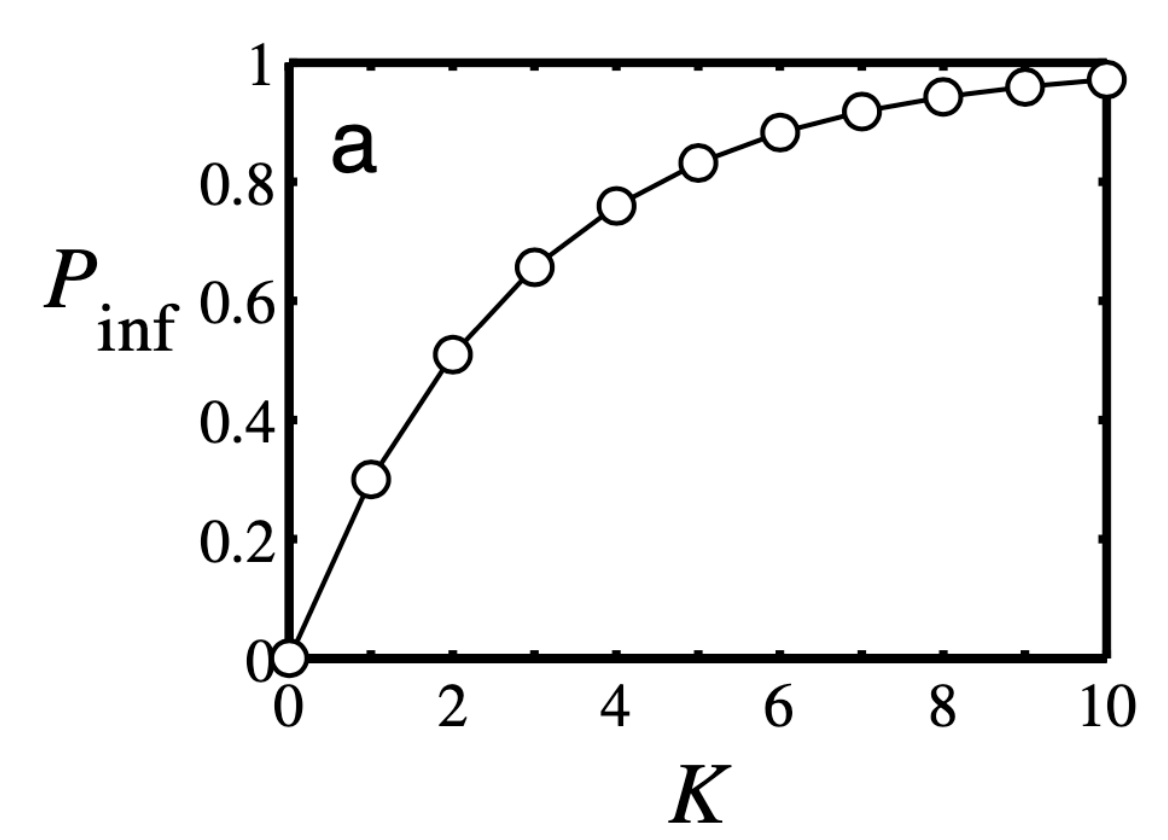
\includegraphics[width=0.4\textwidth]{../lessons/image/11/1.png}
\caption{\label{fig:11_1} Generalized Complex Contagion model: epidemic spreading.}
\end{figure}


\item if \( p=1 \)  and fixed dose size $f(d) = \delta(d-1)$ and fixed threshold $g(d^*) = \delta(d^*-5)$ we have \textbf{deterministic threshold model}. In particular, the treshold is fixed at \( d^*=5 \), so we need at least 5 encounters to get infected. Hence, the dose size is exactly the same of before (since the distribution is still peaked around one), but I need more than one contact (for instance 5 friends show to me the information). See Fig. \ref{fig:11_2};

\begin{figure}[h!]
\centering
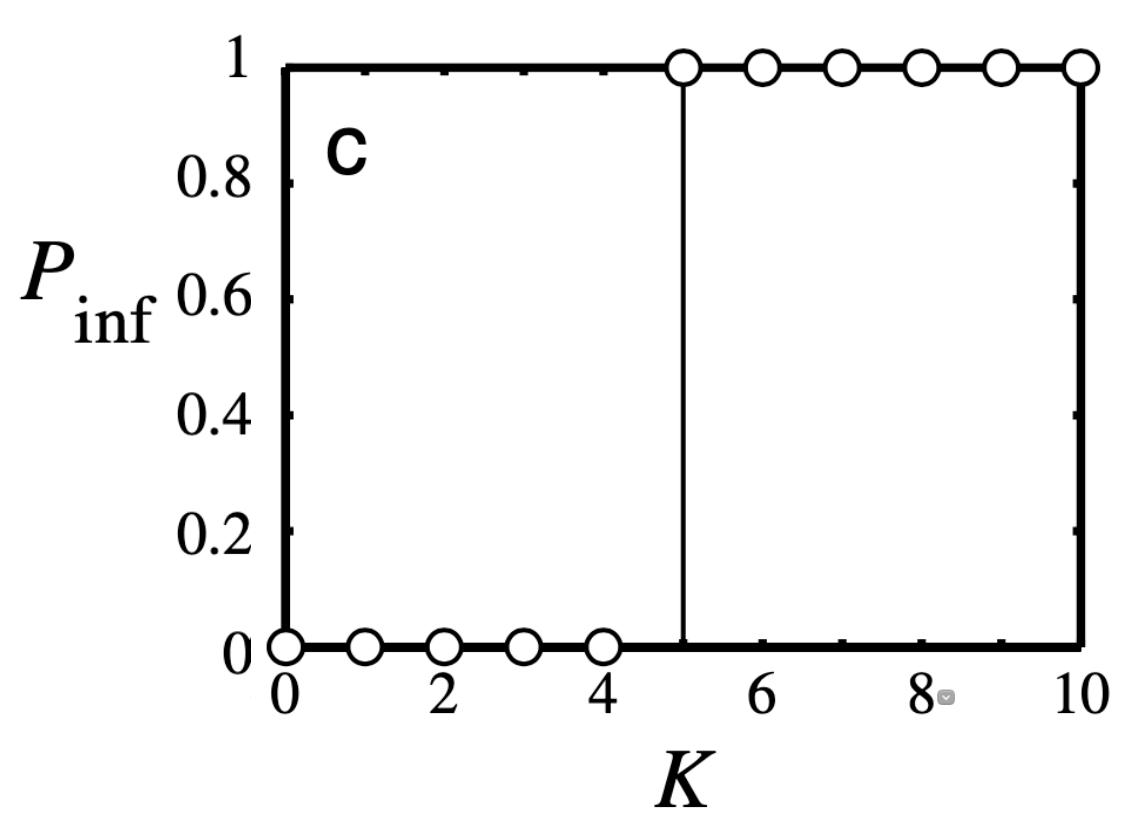
\includegraphics[width=0.4\textwidth]{../lessons/image/11/2.png}
\caption{\label{fig:11_2} Generalized Complex Contagion model: deterministic threshold model.}
\end{figure}

\item if \( p=1 \)  and fixed dose size $f(d)$ is distributed log-normally and fixed threshold $g(d^*) = \delta(d^*-5)$ we have \textbf{stochastic threshold model}. In particular, the treshold is still fixed at \( d^*=5 \), but the “dose” for each contact varies.
Hence in this case we are considering that the contacts are not equal (for instance I trust one friend more tha another) and we get that the threshold is of the same, but the dose size is different. See Fig. \ref{fig:11_3}.

\begin{figure}[h!]
\centering
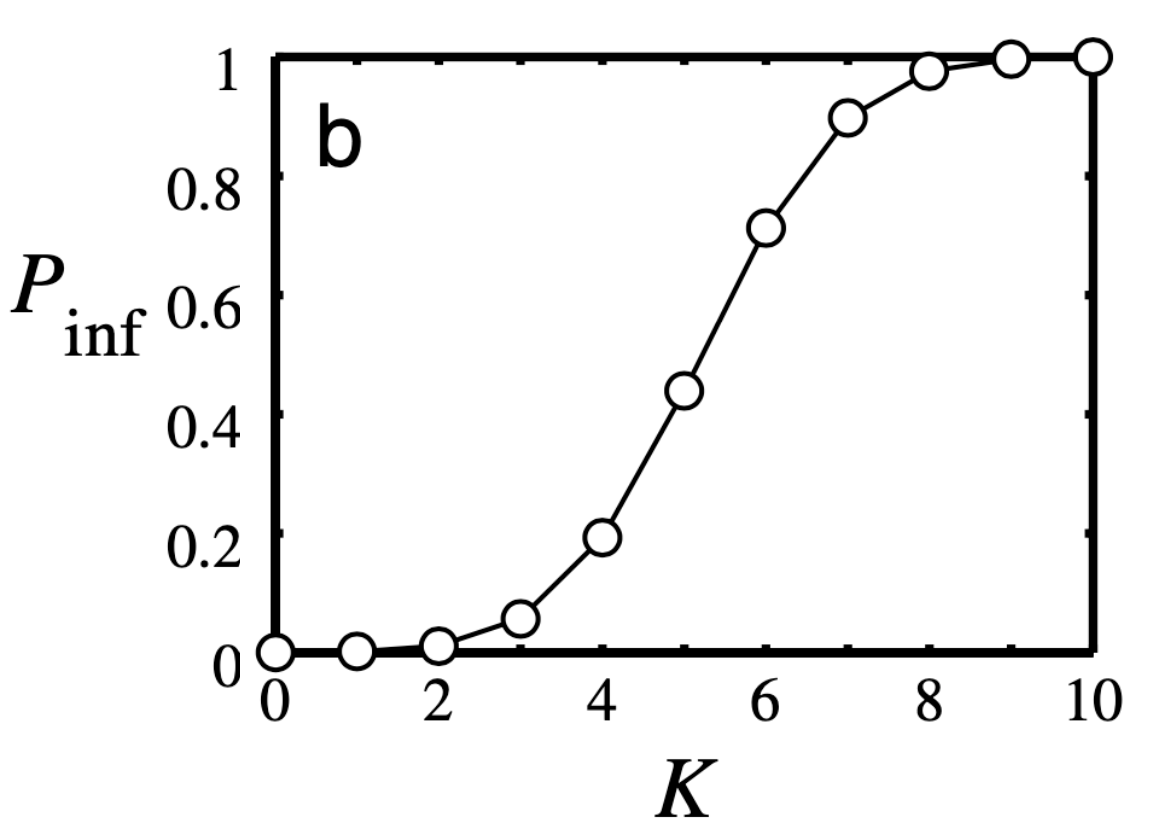
\includegraphics[width=0.4\textwidth]{../lessons/image/11/3.png}
\caption{\label{fig:11_3} Generalized Complex Contagion model: stochastic threshold model.}
\end{figure}

\end{itemize}






\section{Applications to Online Social Networks}

The question is: how hashtags (memes) spread in online social networks?
Let us consider the analysis of real data on Twitter.
In twitter we have different types of commuties. We are gonna study of retweets (RT) and mentions (@) diffuse hashtags in different communities and in particolar we want to see the effect of communities (i.e. how reinforcmenet and homophily will have a role on spreading)

To quantify the fraction of information that flows inside a community and outside, we are gonna use the following weights:
\begin{itemize}
\item \( \expval{w_\circlearrowright}_c  \) is the average weight (number of tweets) per link inside the community;

\item \( \expval{w_\curvearrowright}_c  \) is the average weight (number of tweets) per link outside the community.
\end{itemize}
The same for users activity:
\begin{itemize}
\item \( f_\circlearrowright \) is the fraction of activity inside the community;

\item \( f_\curvearrowright  \) is the fraction of activity outside the community.
\end{itemize}

If information in Twitter spread like a \emph{simple contagion} there should be no differences in spreading inside and outside a community (e.g. \emph{no reinforcement})
Instead, if we see that the average weights inside the community are major than outside actually you need some sort of reinforcment.

In Fig. \ref{fig:11_4} we can see the results showing the average weitgh inside a community and outside. They are pretty similar, but what happens is that it seems that the average are a little bit higher for spreading inside a community (homophily and reinforcment have a role).

\begin{figure}[h!]
\centering
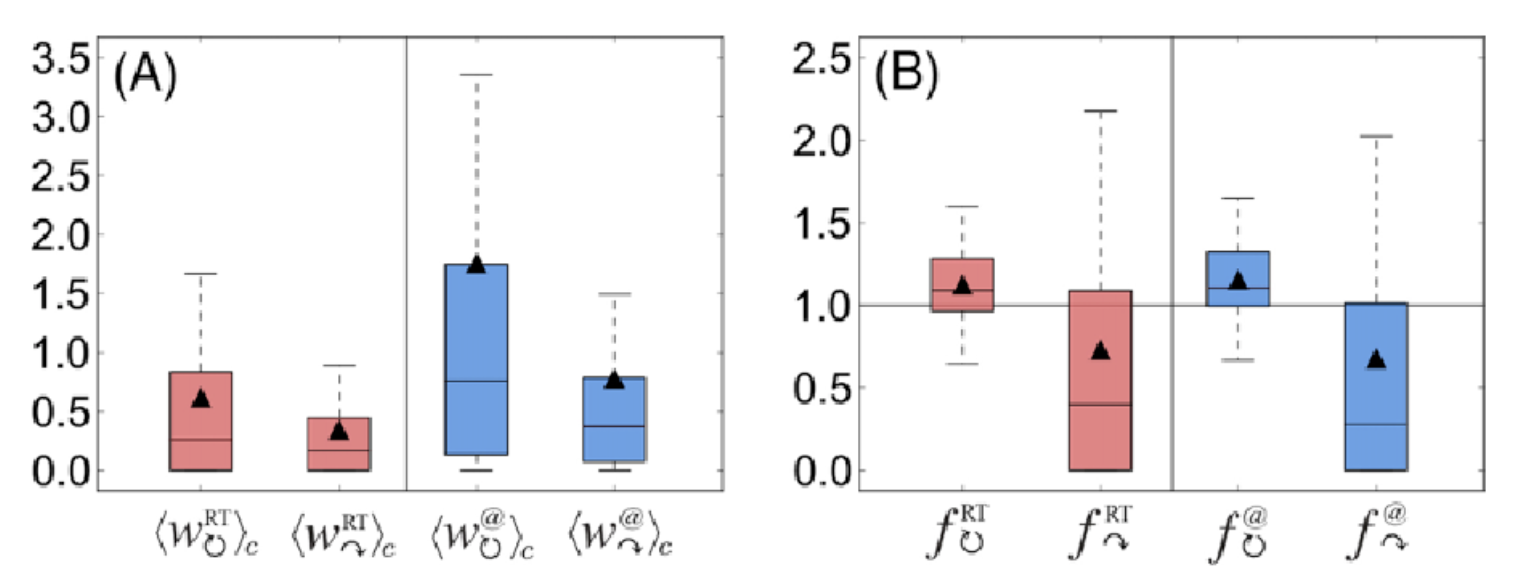
\includegraphics[width=0.8\textwidth]{../lessons/image/11/4.png}
\caption{\label{fig:11_4}  Community spreading is favored (effects of homophily and reinforcement).}
\end{figure}



To clarify that point we introduce more measures at the simple hastag (\( h \)) level: we measure the hashtag inside a community and outside (i.e. for each hastag we measure the popularity that a tweet got). In particular, for each hastag:
\begin{itemize}

\item we measure the \textbf{usage dominance} $r(h)$: proportion of tweets produced inside the “main” community of $h$ out of the total number of tweets
containing $h$, $T(h)$. We expect that this measure is low for viral spreading and high for complex contagion;

\item we measure the \textbf{usage entropy} \( H(h) \): how \( h \) is distributed across communities. It is high for viral spreading and low for complex contagion;

\item we measure the \textbf{average exposure} $N(h)$: average number of exposures needed to adopt hashtag $h$. It is low for viral spreading and high for complex contagion.

\end{itemize}

We have some reference models (4 models \( M_{1, \dots,4} \)) to represent dofferent baseline behavior (see Fig. \ref{fig:11_5} for more details):

\begin{itemize}
\item the simplest one is when for a given hastag \( h \), the model \( M_1 \) randomlu samples the same number of tweets or users as in the real data (i.e. data are extracted at random). We got some sort of \textbf{average behavior} for all the hastags (no community, no network structure);

\item the second model is just an epidemic model. In particular, \( M_2 \) takes the \emph{network structure} into account while neglecting social reinforcement and homophily.  Each hastag starts with a random users and at each step with a certain probability spread to the other user. This is a reference model for \textbf{simple contagion};

\item we can have more complex model which takes into account the \emph{network structure}, \emph{reinforcement} and \emph{homophily}.  This is a reference model for \textbf{complex contagion}.
\end{itemize}

\begin{figure}[h!]
\centering
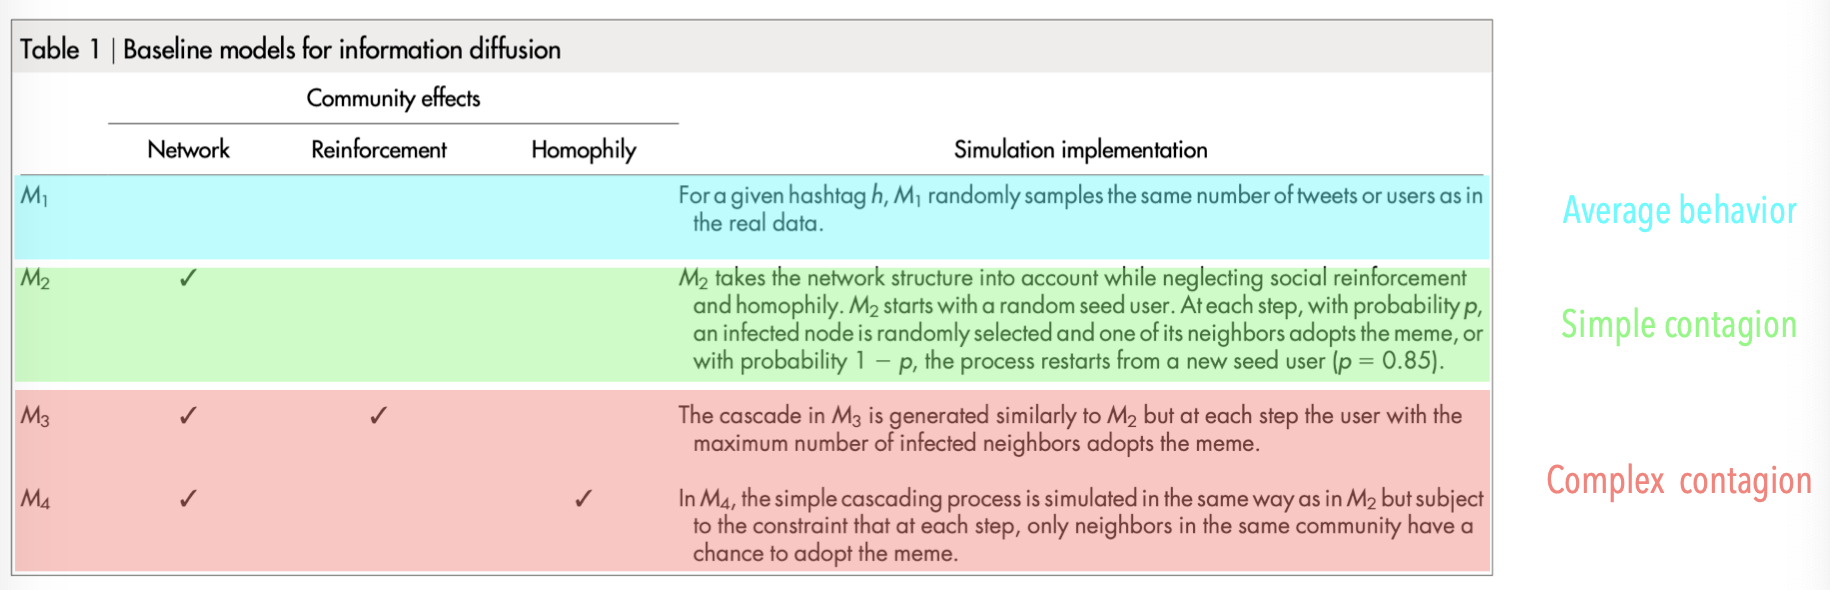
\includegraphics[width=0.9\textwidth]{../lessons/image/11/5.png}
\caption{\label{fig:11_5} Reference models for information spreading in online social networks.}
\end{figure}

Let us consider Fig. \ref{fig:11_6} where we can see \( r(h) \), \( H(h) \) and \( N(h) \) as function of the number of tweets \( T \) and the number of users \( U \).
The black lines represent the real data, the dashed lines represent model \( M_1 \) (average behavior), the red square \( M_2 \) (simple contagion) while the blue and green models \( M_3 \) and \( M_4 \) (complex contagion).

There is a real distinction between popular (in grey) and not popular hastags.
We see two main behaviors:
\begin{itemize}
\item popular hashtags (large $T$ and $U$) spread like epidemics (viral);
\item less popular ones follow a complex contagion.
\end{itemize}



\begin{figure}[h!]
\centering
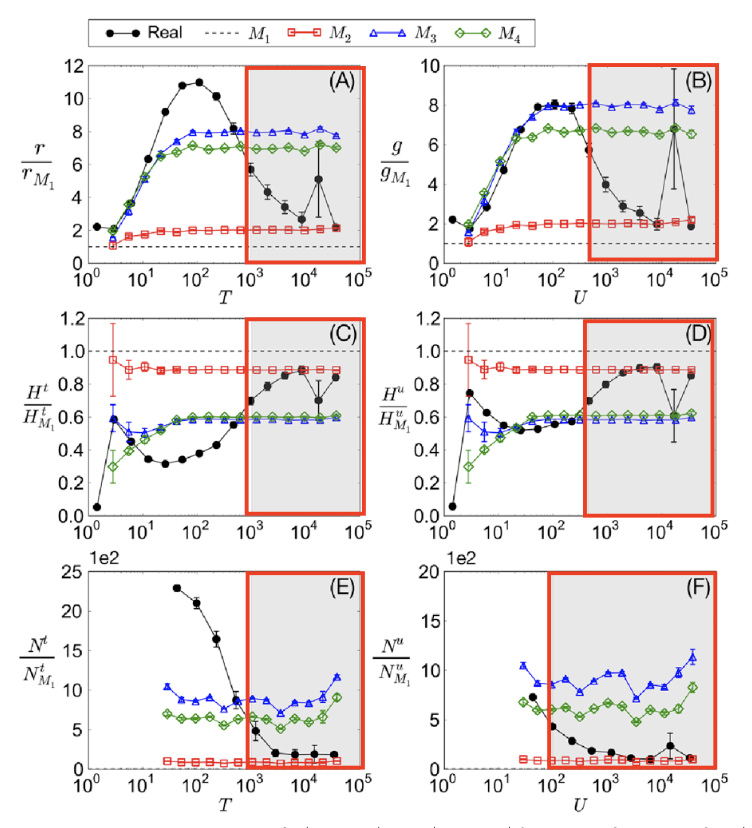
\includegraphics[width=0.9\textwidth]{../lessons/image/11/6.png}
\caption{\label{fig:11_6} Results of information spreading in online social networks.}
\end{figure}




















\end{document}
